\documentclass[12pt]{article} 
\usepackage[margin=1in]{geometry}
\usepackage{enumitem} %% for custom list
\usepackage{graphicx} %% for images
\usepackage{multirow} %% for tables
%\usepackage{bigints}  %% for BIG integrals
\usepackage{bytefield} %% for drawing packet structure
\usepackage{amsmath}
\usepackage[load-configurations = abbreviations]{siunitx}

% used for tabbed spacing
%\newcommand{\itab}[1]{\hspace{0em}\rlap{#1}}
%\newcommand{\tab}[1]{\hspace{.4\textwidth}\rlap{#1}}



% using \code{come code monospaced}
\def\code#1{\texttt{#1}}

\begin{document}
\date{}
%\author{Andrea Ghizzoni \\
%some other info}
\title{\vspace{-11ex}} %% used for no title
 
\maketitle

\section{Il Livello Trasporto}\label{livello-trasporto}
I protocolli di livello Trasporto forniscono la comunicazione logica tra processi 
applicativi, detta anche comunicazione \textit{end-to-end}. 

Il suo obiettivo \'e quello di frammentare e riordinare i segmenti inviati e ricevuti, fornendo un livello di 
astrazione superiore che permetta ai processi applicativi di usare la rete sottostante senza conoscerne ne la 
topologia ne la tecnologia sottostante effettivamente utilizzata. Basti pensare che una data applicazione non 
interessa generalmente se i dati vengono inviati tramite frequenze radio o via cavo, a lei interessa che i dati 
arrivino alla destinazione.

Questo servizio non pu\'o essere fornito dai livelli sottostanti perch\'e non prevedono lo stesso livello di 
affidabilit\'a.

Gli obiettivi del livello di trasporto sono stati implementati in due protocolli di base: \textbf{TCP} e 
\textbf{UDP}. La loro caratteristica comune \'e quella di eseguire il \textbf{multiplexing} \textit{(multiplazione)} 
e il \textbf{demultiplexing} \textit{(demultiplazione)} dei dati inviati e ricevuti dalle applicazioni del livello 
superiore, ovvero riconoscere a quale applicazione consegnare, o inviare, il flusso dati in ingresso o in uscita, in 
presenza di una gestione concorrente delle risorse di rete.

A questo livello protocollare la PDU\footnote{\textit{PDU}: Package Data Unit} prende il nome di \textbf{segmento}, 
mentre i livelli superiori lo utilizzano tramite la SAP\footnote{\textit{SAP}: Service Access Point} appropriata, 
chiamata \textbf{TSAP} \textit{(Transport Service Access Point)}.

\subsection{mux/demux}\label{livello-trasporto-mux-demux}
Per eseguire la multiplazione e la demultiplazione dei flussi di dati, il livello di trasporto identifica ogni 
processo tramite un numero intero senza segno su a 16 bit, chiamato \textbf{porta}. L'associazione tra processo e 
numero di porta viene gestito dal sistema operativo, dove risiede l'implementazione del livello trasporto.

Per convenzione i numeri di porta da \code{0-1023} vengono chiamate \textbf{Well-known Port} \textit{(Porte ben 
conosciute)}, ovvero numeri riservati per applicazioni standard, mentre i numeri di porta da \code{1024-65535} sono 
lasciati per tutte le altre applicazioni.

Ovviamente la porta del client, nel momento di stabilire una connessione, pu\'o essere una porta scelta a caso dal 
sistema operativo, cosa non vera per la porta di destinazione, che deve essere appropriata per identificare 
l'applicazione remota.



\clearpage
\section{ARQ - Automatic Retransmission reQuest}\label{arq}
Vengono definiti \textbf{ARQ} \textit{(Automatic Retransmission reQuest)} tutti quei protocolli che consentono di 
richiedere in modo automatico la trasmissione dei segmenti persi o non consegnati.

Ogni ARQ fa uso della tecnica chiamata a \textbf{Sliding Windows} \textit{(Finestre a Scorrimento)}, ovvero usano un 
buffer di PDU inviate e ricevute, e dei segmenti particolari per il riscontro dell'avvenuta ricezione della PDU da 
parte del destinatario, chiamati \textbf{Acknowledgement} \textit{(Riscontro)}; pi\'u formalmente si definisce:

\paragraph{Finestra di Trasmissione $W_t$} come la quantit\'a massima di PDU in sequenza che il trasmettitore \'e 
autorizzato ad inviare in rete senza averne ricevuto nessun riscontro.
	
\paragraph{Finestra di Ricezione $W_r$} come la quantit\'a massima di PDU che il ricevitore pu\'o memorizzare dal 
trasmettitore.

\paragraph{Acknowledgement $ACK(n)$} come il riscontro per il segmento con numero di sequenza uguale a $n$.\\

L'utilizzo delle finestre scorrevoli comporta anche il problema dell'inizializzazione delle stesse ad una dimensione 
appropriata, risolto da TCP al momento della connessione tramite un'apposita procedura.

L'impostazione di una dimensione consona \'e cruciale, in quanto: se troppo grande si rischia di sprecare memoria, 
altrimenti il ricevitore rischia di inviare ACK per ogni pacchetto ricevuto; questo vanifica 
concettualmente tutti i benefici della tecnica a finestre scorrevoli. La dimensione solitamente adottata \'e quindi 
\begin{center}
	$W_r = W_t$.
\end{center}

\begin{center}
	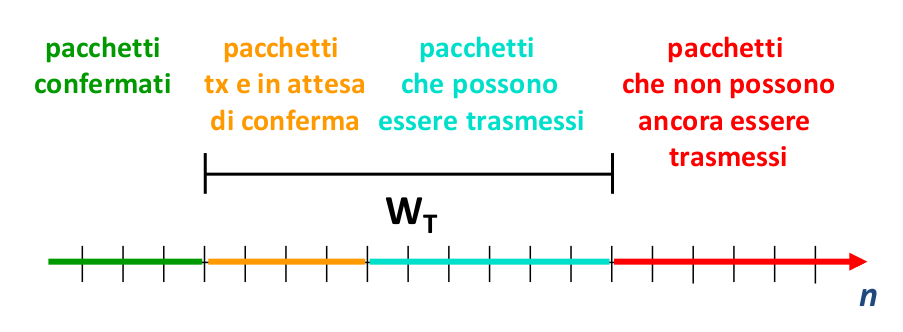
\includegraphics[scale=0.3]{livello_trasporto-img18.png}
\end{center}

\begin{center}
	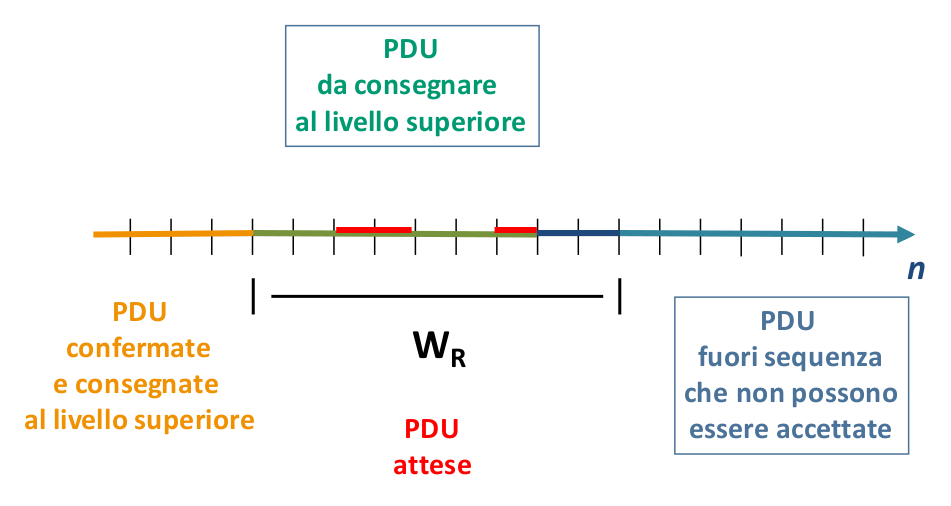
\includegraphics[scale=0.3]{livello_trasporto-img19.png}
\end{center}

Ogni PDU inviata all'interno di una finestra a scorrimento ha un numero di sequenza a \textit{k} bit. 
La numerazione \'e necessaria per tenere traccia dell'ordinamento dei dati in fase di ricezione e serve al 
destinatario per sapere qual'\'e il prossimo segmento da ricevere: nel caso in cui il destinatario riceva un 
segmento fuori dalla sua finestra di ricezione, il segmento verr\'a scartato.

La numerazione segue la numerazione modulo $2^k$ ovvero viene eseguita ciclicamente su k bit.

Attraverso il sistema di ACK \'e possibile implementare il controllo di flusso: basta inserire 
un campo nell'intestazione dei segmenti ACK dove il ricevente specifica la dimensione corrente della 
sua finestra di ricezione, in unit\'a di  PDU del protocollo in uso; in questo modo il trasmettitore non 
invier\'a pi\'u di quello che il ricevente pu\'o gestire.

\subsection{Semantica dei pacchetti di riscontro}\label{arq-semantica-dei-pacchetti-riscontro}
Ogni volta che si instaura una connessione, le due entit\'a devono accordarsi sul significato semantico del pacchetti 
di riscontro ACK, che pu\'o essere:
\begin{itemize}[noitemsep]
	\item \textbf{ACK individuale o selettivo:} assegna ad ogni pacchetto di riscontro un valore,ovvero il numero di 
		  sequenza del segmento riscontrato. Quindi ACK(n) viene inteso come \textit{"ho ricevuto il pacchetto N"}. 
		  Questo prevede che il destinatario mantenga traccia del numero di sequenza del successivo frame che si 
		  aspetta di ricevere, e spedisce tale numero, ogni volta che manda un segnale ACK
	\item \textbf{ACK cumulativi:} assegna ad ogni pacchetto di riscontro un valore ACK(N) che viene inteso come 
	      \textit{"ho ricevuto tutti i pacchetti fino a N escluso"}. In caso di errore per\'o e' necessario    
	      ritrasmettere l'intera finestra in quanto il trasmettitore non ha idea di quale pacchetto sia andato perso 
	      \item \textbf{ACK negativo o NAK:} assegna ad ogni pacchetto di riscontro un valore NAK(N) che viene inteso 
	      come \textit{"ritrasmetti il pacchetto N"}
\end{itemize}

\subsection{Piggybacking}\label{arq-piggybacking}
La tecnica Piggybacking \'e utile nel caso in cui vi siano comunicazioni bidirezionali al fine di
ridurre i pacchetti che viaggiano sulla rete e, di conseguenza, aumentare le prestazioni del
protocollo.

Con questa tecnica gli ACK, non vengono spediti come un segmento singolo, ma vengono inseriti nell'intestazione delle 
PDU che viaggia nella direzione opposta.

\clearpage
\subsection{Prestazioni dei Protocolli a Finestre}\label{arq-prestazioni-protocolli-finestre-scorrevoli} 
Si definisce \textbf{round trip time} come il doppio del tempo di propagazione:
\begin{equation}\label{eq:rtt}
	RTT = 2 * T_{prop} = 2 * [s]
\end{equation}
Si definisce \textbf{tempo di trasmissione} come il rapporto tra lunghezza del pacchetto $L$ e la capacit\'a della 
rete $R$:
\begin{equation}\label{eq:t-transm}
\begin{split}
	T_{trasm} &= \frac{L}{R} = \frac{[bit]}{[bit/s]} = [s] \\
	T_{trasm} &= \frac{L * 8}{R} = \frac{[byte] * 8}{[bit/s]} = \frac{[bit]}{[bit/s]} = [s]
\end{split}
\end{equation}
Si definisce \textbf{efficienza} o \textbf{utilizzo} come il tempo in cui il mittente \'e occupato nell'invio di bit 
($W_t$ si intende in numero di PDU inviate):
\begin{equation}\label{eq:u-mitt}
	U_{mitt} = \frac{W_t * T_{trasm}}{RTT+T_{trasm}} = \frac{[s]}{[s]}
\end{equation}
Si definisce \textbf{throughput} come la capacit\'a di un algoritmo dell'utilizzo effettivo del mezzo trasmissivo.
Nel caso dell'utilizzo di finestre statiche si definisce throughput:
\begin{equation}\label{eq:throughput-statiche}
\begin{split}
	Thr &= \frac{W_t}{RTT} = \frac{[bit]}{[s]} = \num{}\,\si{bps} \\
    Thr &= \frac{W_t * 8}{RTT} = \frac{[byte] * 8}{[s]} = \frac{[bit]}{[s]} = \num{}\,\si{bps}
\end{split}
\end{equation}
Nel caso invece di finestre di dimensione variabile si ottiene:
\begin{equation}\label{eq:throughput-dinamiche}
    Thr = \int_{T_{trasm}} W_{t}(t) dt = \frac{[bit]}{[s]} = \num{}\,\si{bps}
\end{equation}
\paragraph{Esempio:}\label{para:esempio-finestre} collegamento a 1 Gbps, pacchetti da 8 kbit, ritardo di propagazione 
di 15 ms e finestra scorrevole pari a 1 PDU, quindi:
\begin{equation}\label{eq:esempio-finestre-wr1}
\begin{split}
	T_{trasm} &= \frac{\num{8}\,\si{kbit}}{\num{d+9}\,\si{bps}} = 0.008 \\
	Thr &= \frac{\num{8}\,\si{kbit}}{\num{0.03}\,\si{\s}} =  \num{266}\,\si{kbps} \\
	U_{mitt}  &= \frac{0.008}{(\num{15}\,\si{\s}*2) + 0.008} = 0.00027
\end{split}
\end{equation}
Nel caso in cui si abbia una finestra scorrevole pi\'u grande, ad esempio $W_r = 3$ si ottiene:
\begin{equation}\label{eq:esempio-finestre-wr3}
	U_{mitt} = \frac{3 * 0.008}{(\num{15}\,\si{\s}*2) + 0.008} = 0.0008
\end{equation}
Aumentando la finestra scorrevole si ottiene un aumento del tempo in cui il mittente \'e occupato nell'invio 
dei bit, quindi un aumento dell'efficienza.

\subsection{Stop and Wait}\label{arq-stop-and-wait}
I protocolli di trasporto a finestra scorrevole di tipo Stop and Wait funzionano nel seguente modo:
\begin{itemize}[noitemsep]
	\item Trasmettitore:
	\begin{itemize}[noitemsep]
		\item invia una PDU[$SEQ\footnote{Il campo \textit{Sequence Number} nell'intestazione di TCP}=X$] e ne salva 
		      una copia. $X$ \'e il numero di SEQ dell'ultimo ACK
		\item attiva un timer ad un tempo standard
		\item si pone in attesa della ricezione del ACK[$SEQ=X+1$]
		\item se riceve l'ACK[$SEQ=X+1$], la procedura ricomincia
		\item se scade il timer, ritrasmette la PDU 
	\end{itemize}
	\item Ricevitore
    \begin{itemize}[noitemsep]
    		\item riceve una PDU
    		\item calcola il checksum e lo confronta con quello nell'intestazione della PDU; se fallisce scarta la PDU
    		\item se $SEQ == X\footnote{Il numero di sequenza viene accordato in fase di connessione}$ allora \'e la PDU 
    		      attesa, altrimenti la scarta
		\item invia ACK[$SEQ=X+1$] e la procedura ricomincia
	\end{itemize}
\end{itemize}

\begin{center}
	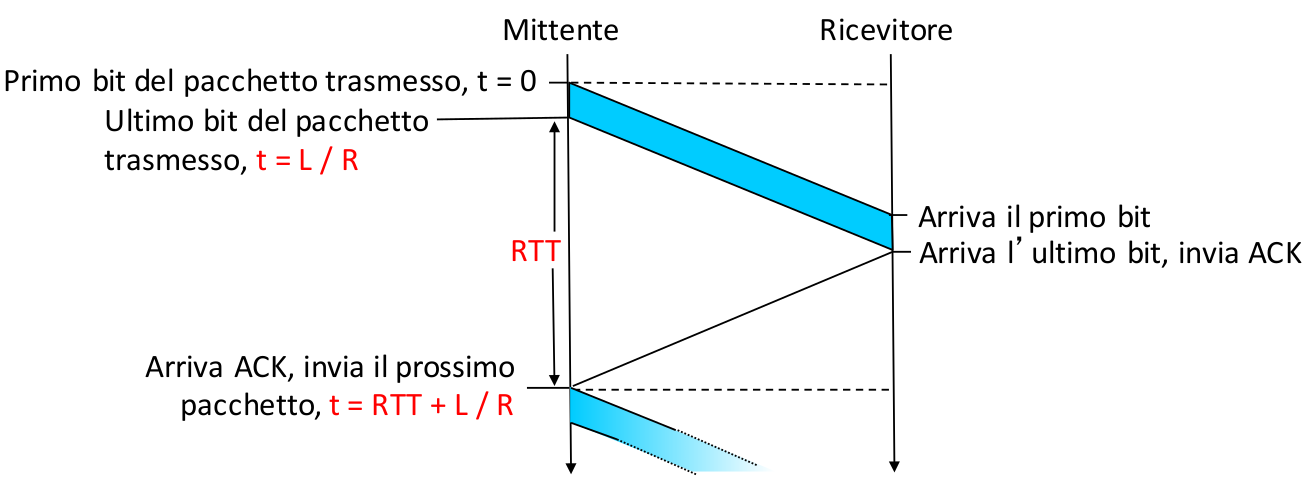
\includegraphics[scale=0.35]{livello_trasporto-img1.png}
\end{center}

Il protocollo \'e poco efficiente perch\'e per ogni PDU inviata dal trasmettitore \'e richiesto un riscontro con un 
ACK. La soluzione \'e l'invio in pipeline delle PDU, ovvero una trasmissione in sequenza.

\clearpage
\subsection{Go Back N}\label{arq-go-back-n}
Questa particolare istanza di ARQ permette di inviare una serie di segmenti, presenti nella finestra dei 
trasmettitore, senza averne prima ricevuto un ACK. 

Nel caso in cui il destinatario non riceva un segmento, continuer\'a a rispondere con ACK duplicati. Una volta che il 
mittente ha esaurito la sua finestra di invio, controlla gli ACK e, se non sono in sequenza, riparte a trasmettere 
dall'ultimo segmento non pervenuto.

\begin{itemize}[noitemsep]
	\item Trasmettitore:
	\begin{itemize}[noitemsep]
		\item invia $N=W_t$ PDU facendo di ognuna una copia
		\item attiva un solo timer per N PDU
		\item si pone in attesa della ricezione degli ACK
		\item se il timer scade, ritrasmette tutte le PDU nella finestra di cui non ha ricevuto un nessun ACK
		\item se riceve un set di ACK con $SEQ=X$, dove X \'e il pi\'u piccolo numero di sequenza dei segmenti che 
		      sono stati trasmessi, allora procede alla ritrasmissione di tutti i segmenti con campo $SEQ \geq X$
	    \item al contrario, se riceve un ACK per ogni segmento che ha nella finestra, la procedura ricomincia
	\end{itemize}
	\item Ricevitore
    \begin{itemize}[noitemsep]
        \item riceve una PDU
   		\item calcola il checksum e lo confronta con quello nell'intestazione della PDU; se fallisce scarta la PDU
		\item se la PDU contiene il primo numero di SEQ non ancora ricevuto, allora risponde con un ACK contenente il 
		      successivo numero di sequenza atteso, altrimenti scarta l'intera PDU. Ricomincia la procedura
	\end{itemize}
\end{itemize}

\subsection{Selective-Repeat}\label{arq-selective-repeat}
Il protocollo Selective Repeat sopperisce alle mancanze di Go-Back-N in termini di prestazioni. Prevede infatti che 
il destinatario accetti le PDU fuori sequenza, ma comunque all'interno della finestra di ricezione, e ne invii i 
rispettivi riscontri.

\begin{itemize}[noitemsep]
	\item Trasmettitore:
	\begin{itemize}[noitemsep]
		\item invia $N=W_t$ PDU facendo di ognuna una copia
		\item attiva un timer per ogni PDU
		\item quando riceve	un ACK relativo ad una PDU la toglie dalla finestra di trasmissione e trasmette una 
		      nuova PDU
		\item se scade il timer, ritrasmette la PDU relativa, facendo partire un nuovo timer
	\end{itemize}
	\item Ricevitore
    \begin{itemize}[noitemsep]
        \item riceve una PDU
   		\item calcola il checksum e lo confronta con quello nell'intestazione della PDU; se fallisce scarta la PDU
   		\item se il numero di sequenza SEQ della PDU \'e contenuto all'interno della finestra di 
   		      ricezione, allora risponde con i relativi riscontri, altrimenti la scarta.
	\end{itemize}
\end{itemize}



\section{TCP}\label{tcp}
TCP \textit{(Transmission Control Protocol)} \'e stato progettato appositamente per fornire un servizio affidabile 
su una rete chiaramente inaffidabile. \'E compito di TCP stabilire una connessione full duplex\footnote{full duplex: 
vengono aperte due "mezze" connessioni in entrambe le direzioni}, spedire i dati, riscontrare l'avvenuta ricezione, 
ritrasmettere i dati in caso di perdita e riordinarli nel caso in cui non arrivino in ordine.

Le entit\'a TCP scambiano dati sotto forma di \textbf{segmenti}, che sono composti da: 20 byte di intestazione
\textit{(header)} e da 0 a 1460 byte di dati \textit{(payload)}, chiamata 
\textbf{MSS} \textit{(Maximun Segment Size)}. Quest'ultima dimensione \'e vincolata per 
convenzione dalla dimensione massima dei segmenti che possono essere trasmessi su una rete ethernet, ovvero 1500 
byte\footnote{1500 byte trama ethernet = 20 header IP + 20 byte header TCP + 1460 byte payload (default MSS)}. 
Ulteriormente esiste un vincolo che riguarda l'incapsulamento  dei segmenti nei 
pacchetti IP, che deve rispettare le dimensioni del payload, chiamato \textbf{MTU} \textit{(Maximun 
Transfer Unit)}. In Pratica ogni MTU definisce il limite superiore per la dimensione di un segmento 
che pu\'o circolare su una data rete. Pu\'o succedere che delle reti, connesse tra di loro, abbiano MTU differenti, 
di conseguenza c'\'e bisogno di scoprire la minima MTU sul tratto di rete. Questa limitazione \'e quindi una chiara 
violazione del principio di indipendenza e stratificazione del modello protocollare.

A questo proposito si utilizzano protocolli di \textbf{MTU path discovery} attraverso messaggi di controllo 
\textbf{ICMP} \textit{(Internet Control Message Protocol)} i quali testano la rete sottostante con segmenti di 
dimensione incrementale fino a quando i segmenti vengono persi.

TCP implementa anche un meccanismo di controllo degli errori sull'intero segmento (pi\'u 8 byte dell'header del 
livello sottostante, contenenti l'indirizzo sorgente e destinazione a livello IP) tramite il 
calcolo di un \textit{checksum} a 16 bit. Il mittente, una volta formato il segmento, aggiunge all'intestazione il 
checksum relativo nell'apposito campo e procede all'invio; il destinatario invece, calcoler\'a il checksum nello 
stesso modo e lo confronter\'a con quello contenuto nell'intestazione del segmento appena ricevuto. Se il confronto 
porta delle differenze tra i codici di controllo TCP scarta completamente il segmento e ne chiede la ritrasmissione.

\subsection{TCP in breve}
\begin{itemize}[noitemsep]
	\item mantiene lo stato della connessione: si occupa dell'instaurazione e del rilascio 
	\item recupero degli errori sul segmento
	\item consegna ordinata dei segmenti all'applicazione
	\item controllo di flusso: controlli per evitare che il \textit{destinatario} non riesca
          a immagazzinare tutti i dati che sto trasmettendo
	\item controllo di congestione: controlli per evitare che la \textit{rete} non riesca a
          consegnare tutti i dati che sto trasmettendo
\end{itemize}

\clearpage
\subsection{Formato del Segmento}\label{tcp-formato-del-segmento}
Il segmento TCP \'e cos\'i composto:
\begin{center}
\begin{bytefield}[boxformatting={\centering},bitwidth=1.0em, bitheight=2em]{32}
	\bitheader{0,15,16,31} \\
	\begin{rightwordgroup}{header\\20 byte}
		\bitbox{16}{Porta Sorgente} & \bitbox{16}{Porta Destinazione}\\
		\bitbox{32}{Numero di Sequenza}\\
		\bitbox{32}{Numero di Riscontro}\\
		\bitbox{4}{Lung Int} & \bitboxes{1}{
			{\tiny C\\W\\R} {\tiny E\\C\\E} {\tiny U\\R\\G} {\tiny A\\C\\K} 
			{\tiny P\\S\\H} {\tiny R\\S\\T} {\tiny S\\Y\\N} {\tiny F\\I\\N}
		} & \bitbox{4}{Riservati} & \bitbox{16}{Finestra di Ricezione}\\
		\bitbox{16}{Checksum} & \bitbox{16}{Puntatore a Dati Urgenti}
	\end{rightwordgroup}\\
	\begin{leftwordgroup}{payload\\0-1460\\byte}
		\wordbox{1}{Opzioni} \\
		\wordbox[]{1}{$\vdots$} \\[1ex]
		\wordbox{2}{Dati}
	\end{leftwordgroup}
\end{bytefield}
\end{center}

\begin{itemize}[noitemsep]
    \item \textbf{Porta Sorgente e Destinazione}: numero di porta sorgente e destinazione.
    \item \textbf{Numero di Sequenza}: numero di sequenza a numerazione ciclica su 32 bit.
    \item \textbf{Numero di Riscontro}: numero usato per il riscontro del segmento, ha significato se il bit 
          \code{ACK} \'e impostato.
    \item \textbf{Lunghezza dell'Intestazione}: numero che rappresenta quanti gruppi di word a 32 bit sono presenti 
          nell'header, in quanto sono presenti opzioni facoltative.
    \item Serie di bit:
    \begin{itemize}[noitemsep]
        \item \code{CWR}: \textit{Congestion Windows Reduce}, se impostato indica di ridurre la congestione
        \item \code{ECE}: \textit{Explicit Congestion Notification}, se impostato indica che l'host supporta questa 
              funzione durante il three-way handshake      
        \item \code{URG}: \textit{Urgent Pointer}, se impostato abilita il campo Urgent Pointer dell'header
        \item \code{ACK}: \textit{Acknowledgement}, se impostato abilita il campo Acknowledgement dell'header
        \item \code{PSH}: \textit{Push}, se impostato indica di passare i dati direttamente all'applicazione
              senza usare buffer di lettura. Usato principalmente nelle applicazioni di terminali 
              remoti
        \item \code{RST}: \textit{Reset}, usato principalmente per rilasciare la connessione in modo netto,
              nel caso in cui il peer non risponda pi\'u
        \item \code{SYN}: \textit{Synchronize}, flag utilizzato per sincronizzare i numeri di sequenza durante
              l'apertura di una connessione. 
        \item \code{FIN}: \textit{Fine}, usato per la chiusura della connessione
    \end{itemize}
    \item \textbf{Finestra di Ricezione}: indica la dimensione della finestra di ricezione del mittente.
    \item \textbf{Checksum}: campo per il controllo degli errori.
    \item \textbf{Dati Urgenti}: rappresenta un offset sui dati del segmento ed indica che quel set di
          dati deve essere consegnato all'applicazione non in ordine con gli alti.
    \item \textbf{Opzioni}: opzioni aggiuntive in word da 32 bit.
\end{itemize}

\subsection{Instaurazione di una Connessione}\label{tcp-instaurazione-connessione}
L'instaurazione della connessione tra entit\'a TCP avviene tramite un processo chiamato \textbf{Three-way 
Handshake} \textit{(Stretta di mano a tre)}.

\begin{center}
	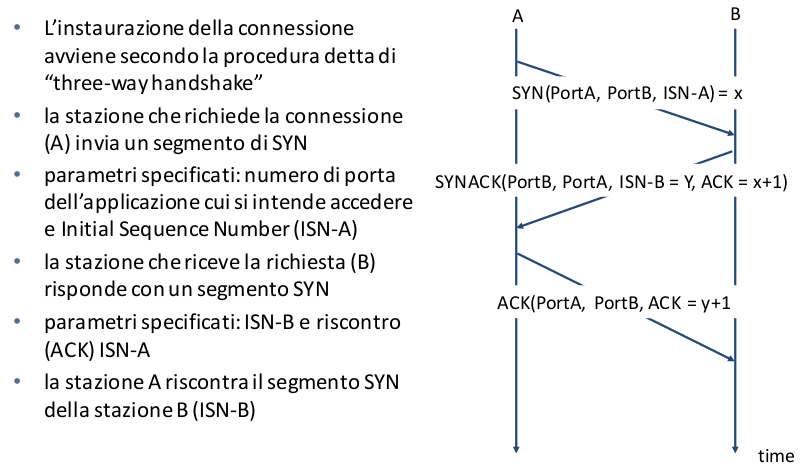
\includegraphics[scale=0.45]{livello_trasporto-img3.png}
\end{center}

Il protocollo di connessione Three-way Handshake prevede lo scambio di segmenti chiamati: \code{SYN}, \code{SYNACK} 
e \code{ACK}, ovvero normali segmenti TCP con i bit \code{SYN} e \code{ACK} attivi.

Con questa procedura \'e possibile che si verifichino delle situazioni indesiderate, dove o il mittente o il 
destinatario ricevono segmenti duplicati.

Nel caso in cui l'host A riceva un segmento con i bit \code{SYNACK} ma, senza aver inviato nessun segmento 
\code{SYN} verso l'host mittente B, allora A provveder\'a ad inviare un segmento con il flag \code{RST} impostato 
per terminare la connessione. Lo stesso comportamento si verifica con la ricezione di segmenti \code{ACK} senza 
prima aver inviato segmenti con numero di sequenza $SEQ=ACK(SEQ-1)$, ovvero senza aver inviato prima il relativo 
segmento.

Nell'ultimo caso, invece, se le due entit\'a tentano di creare una connessione simultaneamente, ne viene creata solo 
una.

\begin{center}
	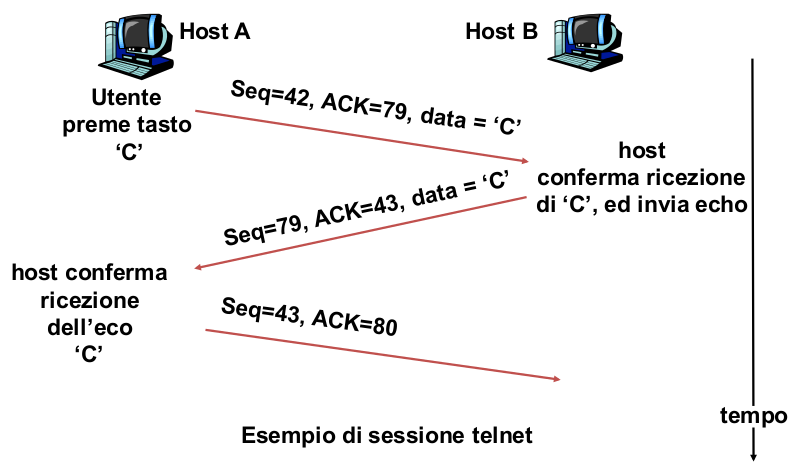
\includegraphics[scale=0.4]{livello_trasporto-img2.png}
\end{center}

\subsection{Chiusura di una Connessione}\label{tcp-chiusura-connessione}
Per rilasciare una connessione entrambe le entit\'a devono inviare e riscontrare un segmento TCP con il flag di 
\code{FIN} impostato, anche chiamato segmento \textbf{DR} \textit{(Disconnection Request)}.

Al momento della ricezione del relativo \code{ACK} la direzione viene chiusa per i nuovi dati, ma possono comunque 
arrivare dati nella direzione opposta. Con questo meccanismo le due parti coinvolte dovranno inviare segmenti 
\code{DR} e attendere l'\code{ACK} per terminare la propria parte di connessione.

In altre parole: quando un host riceve un segmento \code{DR} s\'a che la connessione nel lato opposto \'e terminata 
(non ricever\'a pi\'u dati in quella direzione), ma potr\'a comunque finire di trasmettere i propri dati e terminarli 
con l'invio di un segmento \code{DR} a sua volta

Nel caso un cui venga perso il segmento \code{DR}, l'host in attesa del riscontro, andr\'a in timeout e proceder\'a 
con il ri-invio del segmento.

Nel grafico seguente sono riportati i segmenti \code{FIN} (corrispondenti ai \code{DR}) e i \code{FINACK}, che sono
i riscontri dei segmenti \code{FIN}.
\begin{center}
	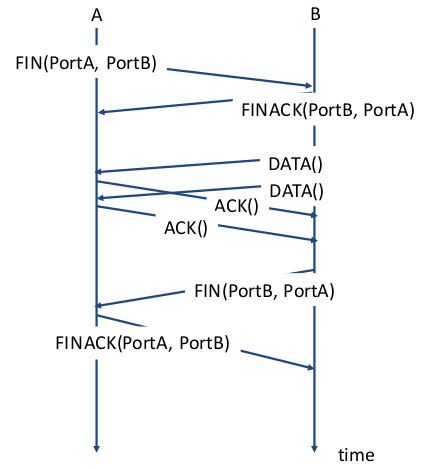
\includegraphics[scale=0.4]{livello_trasporto-img4.png}
\end{center}

\'E possibile terminare la connessione anche impostando il flag \code{RST}. In questo modo la chiusura avviene 
unilateralmente, senza necessit\'a di conferme da nessun lato. \'E molto utilizzata dai server che hanno bisogno di 
liberare le risorse usate dalla connessione in modo rapido, ad esempio per prevenire attacchi di \textit{Denial of 
Service}: l'entit\'a attaccante, dopo aver creato una connessione col server, non risponder\'a mai con i riscontri ai  
segmenti \code{DR}, quindi il server non riusci\'a mai a chiudere il suo lato di connessione e, di conseguenza, non 
liberer\'a mai le risorse a lei assegnate.

\clearpage
\subsection{Gestione dei Timer - Timeout}\label{tcp-timeout}
In TCP sono implementati molti meccanismi che permetto la ritrasmissione dei segmenti nel caso non vengano 
consegnati; ma l'ultima tecnica che possiede (ed \'e l'unica che funziona sempre) \'e quella di utilizzare un timer
chiamato \textbf{RTO} \textit{(Retransmission Time Out)} che, alla scadenza, ri-invia il segmento perso.

Il RTO indica, quindi, il tempo entro il quale la sorgente si aspetta di ricevere un ACK. Questo tempo non pu\'o 
essere impostato staticamente, per via della differenza delle reti fisiche su cui TCP deve basarsi, ma deve tenere 
conto di molti fattori come: la distanza tra sorgente e destinazione, dalla condizione della rete, dalla 
disponibilit\'a dell'host ecc.

Quindi l'unico modo \'e quello di stimare il RTO misurando il tempo trascorso tra l'invio di un segmento e il suo 
riscontro; questo tempo viene chiamato \textbf{RTT} \textit{(Round Trip Time)}.

Il RTT varia da pacchetto a pacchetto, quindi adattare staticamente il RTO a questi cambiamenti improvvisi non \'e 
la scelta migliore.
A questo scopo si utilizza una media mobile esponenziale chiamata \textbf{SRTT} \textit{(Smoothed RTT)}, calcolata e 
tenuta costantemente aggiornata nel seguente modo:
\begin{equation}\label{eq:srtt}
	SRTT = (1-\alpha) \cdotp SRTT + \alpha \cdotp1 RTT
\end{equation}
dove $\alpha$ \'e tipicamente impostata a $1/8$ \footnote{\label{note1}Questa scelta \'e dovuta ad una serie di test 
che hanno riscontrato che \'e un valore appropriato.}. 

In generale, il problema di usare una media come "rappresentante" di un insieme di valori \'e che si perde 
l'informazione di quanto i dati si discostano tra di loro, quindi in questo caso la media non segue fedelmente il 
RTO. 

A questo proposito si utilizza la varianza della madia, chiamata \textbf{RTTVAR} \textit{(Varianza della media SRTT)} 
calcolata nel seguente modo:
\begin{equation}\label{eq:rttvar}
	RTTVAR = (1-\beta) \cdotp RTTVAR + \beta \cdotp \mid SRTT-RTT \mid
\end{equation}
dove $\beta$ \'e tipicamente impostata a $1/4$ $^{\ref{note1}}$.

Conoscendo lo SRTT e l'RTTVAR si pu\'o impostare correttamente il RTO come segue:
\begin{equation}\label{eq:rto}
	RTO = SRTT + 4 \cdotp RTTVAR
\end{equation}
Da notare che \'e data molta importanza alla variabilit\'a della media. Esiste comunque un valore sotto il quale non 
\'e possibile scendere, ovvero $\approx 200ms$

\clearpage
\subsection{Congestione}\label{tcp-congestione}
Uno dei compiti del livello di Trasporto \'e quello di rilevare e reagire alle congestioni che si verificano sulla 
rete. Le cause di una congestione possono essere molteplici: la velocit\'a di elaborazione dei segmenti di alcuni 
apparati di rete, oppure un eccessivo traffico generato dal trasmettitore che satura la capacit\'a della rete.

L'effetto principale \'e la perdita di segmenti lungo la rete, che quindi, ne causa la ritrasmissione da parte dei 
terminali, innescando un circolo vizioso che, se non gestito, porta inevitabilmente la rete a consegnare solo 
informazioni ritrasmesse, quindi al collasso\footnote{Questo \'e accaduto molte volte ai tempi di ARPANET, 
richiedendo che l'intera rete venisse spenta e progressivamente riaccesa.}.

Questa situazione vista in termini di throughput \'e la seguente: in accordo con la sua definizione (equazione 
\ref{eq:throughput-statiche}) all'aumento del RTT segue un calo del throughput, quindi TCP deve trovare il modo di 
adattare $W_t$ dinamicamente in modo da non ridurlo a zero (nel caso in cui scade il RTO).

L'implementazione adottata \'e quella di creare una finestra logica che condiziona la dimensione di $W_t$ in funzione 
dello stato attuale della rete, tale meccanismo prende il nome di \textbf{CWND} \textit{(Congestion Window)}.

La CWND indica, quindi, il numero di segmenti che il mittente pu\'o inviare senza creare congestione sulla rete; 
nel caso un cui ci siano comunque delle perdite di segmenti, TCP interviene variandone la dimensione e, di 
conseguenza, varia anche la finestra di trasmissione che riduce il tasso di invio dei segmenti.

In TCP la finestra di congestione viene gestita tramite due algoritmi che ne garantiscono una crescita 
controllata nel caso non ci siano perdite, \textbf{Slow Start} e \textbf{Congestion Avoidance}, mentre nel caso 
contrario sono stati ideate tecniche che permettono di recuperare selettivamente i segmenti senza creare 
congestione e lasciando il meccanismo di RTO come ultima risorsa, si tratta di: \textbf{Fast Retransmit} e 
\textbf{Fast Recovery}.

Il recupero allo scadere del RTO viene lasciato come ultima risorsa, da usare solo nel caso in cui le altre tecniche 
hanno fallito. Il motivo principale di questa scelta \'e dettata dal fatto che la ritrasmissione con il RTO \'e 
sempre attuabile e perch\'e riduce drasticamente le prestazioni del trasferimento.

All'inizio della connessione TCP imposta la CWND ad un valore molto basso, tipicamente ad 1 MSS, poi l'aumenta 
secondo le tecniche di Slow Start, fino ad una certa soglia chiamata \textbf{SSTRESH} \textit{(Slow Start 
Threshold)}, poi continua con Congestion Avoidance, fino ad un massimo che \'e dato dal mezzo trasmissivo o dalla 
RWND \textit{(Receiver Window)} del destinatario.

\clearpage
\subsubsection{Slow Start}\label{tcp-congestione-slow-start}
Di seguito viene riportato l'immagine dell'andamento di crescita della CWND con l'algoritmo di Slow Start: i segmenti 
verdi sono stati inviati e riscontrati, quelli gialli sono stati inviati ma non ancora riscontrati, quelli bianchi 
invece non sono stati ancora inviati, la finestra di congestione e' raffigurata in blu.
\begin{center}
	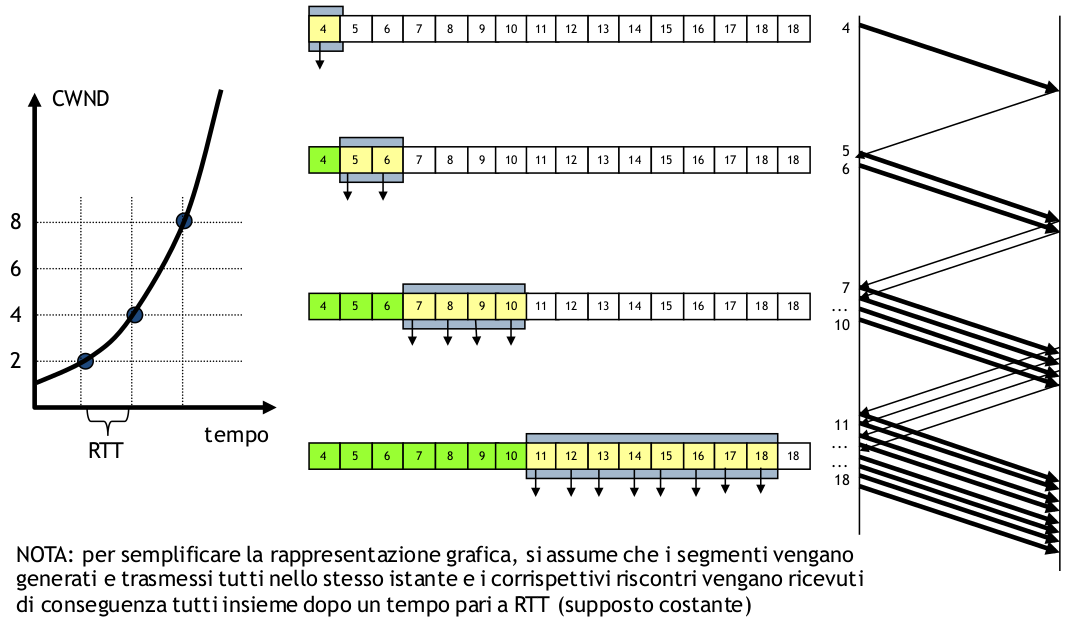
\includegraphics[scale=0.4]{livello_trasporto-img6.png}
\end{center}
Slow Start inizia con la CWND inizializzata ad 1 MSS. Ad ogni ACK (non duplicato) ricevuto (ovvero ad ogni RTT) 
incrementa la finestra di congestione sempre di 1 MSS; questo implica la trasmissione sempre di due nuovi 
segmenti per ACK ricevuto. In altri termini, ad ogni RTT la CWND viene aggiornata nel seguente modo:
\begin{equation}\label{eq:cwnd-slow-start}
	CWND = CWND + MSS
\end{equation}
Questa peculiare caratteristica rende l'evoluzione della dimensione \textit{esponenziale}.

L'inevitabile conseguenza di questo andamento \'e che arriva a saturare il mezzo trasmissivo o la destinazione in 
poco tempo; quindi Slow Start arriva fino alla SSTHRESH dove l'incremento passa a lineare.

\clearpage
\subsubsection{Congestion Avoidance}\label{tcp-congestione-congestion-avoidance}
\begin{center}
	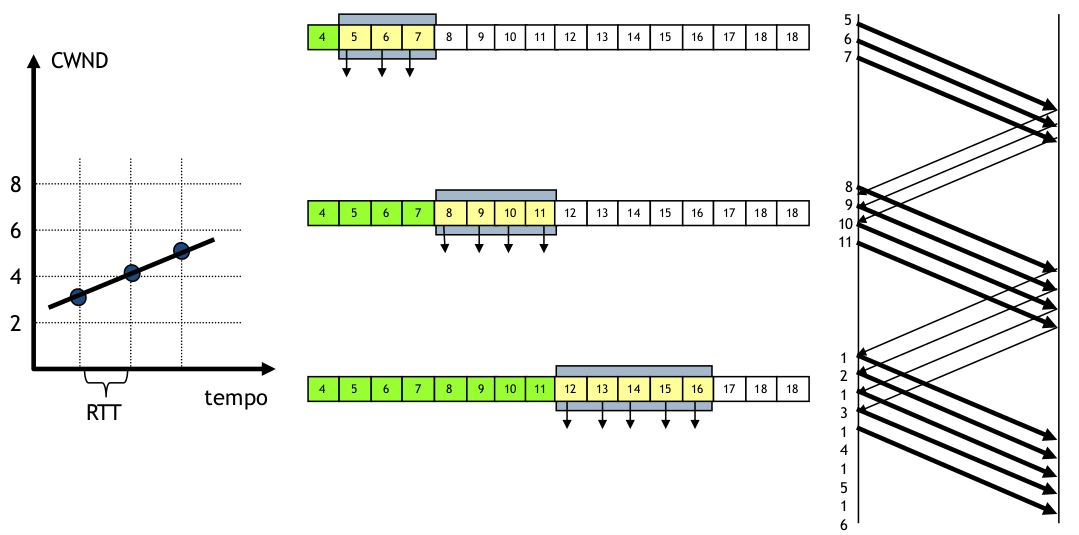
\includegraphics[scale=0.35]{livello_trasporto-img7.png}
\end{center}
L'algoritmo Congestion Avoidance subentra dopo la soglia SSTRESH, per evitare tutti i problemi di Slow Start e
il suo andamento esponenziale.

Congestion Avoidance, ad ogni ACK (non duplicato) ricevuto aumenta la finestra di congestione di un fattore, quindi 
assume un andamento \textit{lineare} ad ogni RTT; ovvero:
\begin{equation}\label{eq:cwnd-congestion-avoidance}
	CWND = CWND + MSS/CWND
\end{equation}
In altri termini: deve ricevere un numero di ACK non duplicati pari ai segmenti presenti nella finestra di 
congestione per aumentarla di 1 MSS.

\subsubsection{Riassumendo}\label{tcp-congestione-riassumendo}
TCP utilizza il seguente algoritmo per evitare la congestione:
\begin{itemize}[noitemsep]
	\item inizio della trasmissione, si pone
	\begin{itemize}[noitemsep]
		\item CWND = 1 segmento, ovvero 1 MSS espresso in byte
		\item SSTRESH = RWND/2		
	\end{itemize}
	\item la CWND evolve secondo l'algoritmo \textbf{Slow Start} fino a SSTRESH
	\item superata la SSTHRESH continua con \textbf{Congestion Avoidance}
	\item la CWND cresce fino al raggiungimento della RWND
\end{itemize}

\begin{center}
	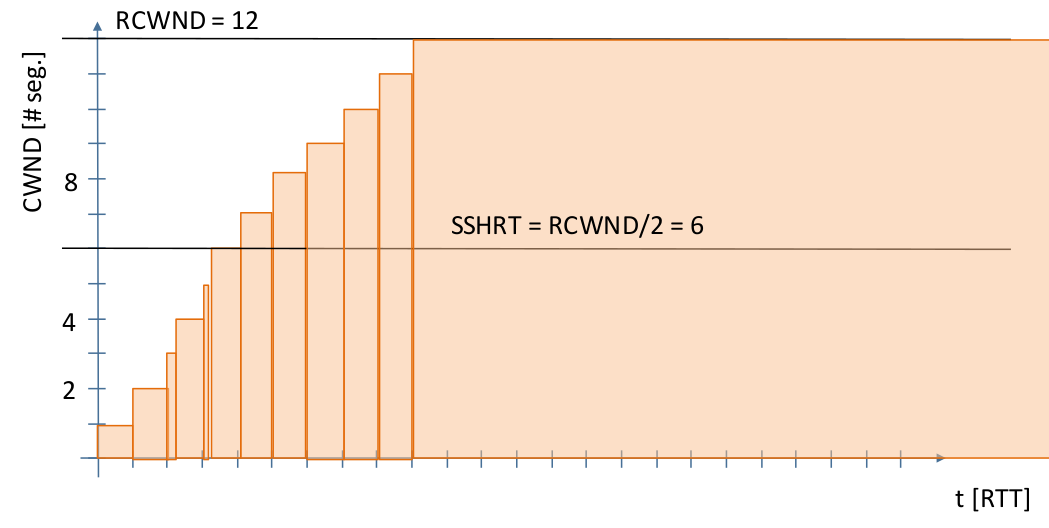
\includegraphics[scale=0.3]{livello_trasporto-img8.png}
\end{center}



\clearpage
\section{Recupero delle Perdite}\label{recupero-delle-perdite}
Durante il normale trasferimento dati \'e possibile che alcuni segmenti vengano scartati dagli apparecchi di rete, 
come router, firewall e gateway, oppure dagli stessi host, per molteplici motivi, il pi\'u frequente \'e l'accumulo 
nei buffer del ricevitore in quanto non riesce a svuotarlo a consegnarli all'applicazione abbastanza velocemente per 
riceverne dei nuovi. 

TCP, una volta rilevato le perdite, utilizza varie tecniche per il recupero di dati; possono variare dall'utilizzo di 
del RTO, oppure da algoritmi pi\'u complessi come Fast Retransmit e/o Fast Recovery che tengono conto dello stato 
della congestione della rete oppure dell'host di destinazione.

Questi algoritmi implementano la specifiche ARQ descritte dei paragrafi precedenti.

\subsection{Recupero con RTO}\label{recupero-delle-perdite-rto}
Il meccanismo pi\'u semplice per il recupero di un segmento non riscontrato \'e quello di lasciar scadere un timer, 
il RTO, e poi procedere alla ritrasmissione. Ad ogni scadenza il RTO viene raddoppiato, lasciando la possibilit\'a 
che la congestione si risolva da sola: si pensi ad un host particolarmente congestionato che deve svuotare i propri 
buffer. La tecnica di raddoppiare il RTO ogni volta che scade viene chiamata \textit{Back-off Esponenziale}. Se scade il RTO per 16 volte, TCP dichiara che non \'e pi\'u connesso alla rete.

Andando in dettaglio, alla scadenza di un RTO avvengono le seguenti azioni:
\begin{enumerate}[noitemsep]
	\item $RTO=RTO \cdotp 2$: raddoppio del valore del precedente RTO, per le ragioni spiegate sopra
	\item $SSTRESH=CWND/2$: viene impostata la soglia di Slow Start a met\'a della finestra di congestione
	\item $CWND=MSS$: viene impostata la finestra di congestione alla dimensione di un segmento
	\item Ritrasmette il primo segmento della finestra: per costruzione, il primo segmento 
	      della finestra di congestione \'e il segmento non riscontrato
	\item Attende il riscontro: in questo caso pu\'o ricevere i seguenti tipi di ACK:
	\begin{itemize}[noitemsep]
		\item se $ACK(SEQ) = W_{low}$ significa che \'e stato perso ancora il segmento appena ritrasmesso, quindi la 
			  procedura riparte dal punto 4
		\item se $W_{low} < ACK(SEQ) < W_{up}$ allora significa che ha riscontrato il segmento perso ed ha 
		      richiesto la ritrasmissione di un altro segmento della finestra anch'esso perso; quindi viene spostato 
		      il bordo inferiore della finestra di trasmissione al numero di SEQ ricevuto: $W_{low} = ACK(SEQ)$
	    \item se $ACK(SEQ) > W_{up}$ allora la ritrasmissione \'e andata a buon fine, tutti i segmenti
	          persi sono stati ricevuti e riscontrati quindi pu\'o riprendere la normale trasmissione
	\end{itemize}
	\item Se scade il RTO: ricomincia la procedura dal punto 1 per 10 volte, poi altre 6 senza aumentare il
	      RTO, poi si arrende.
\end{enumerate}
Da notare che in questo caso si utilizzano ACK comulativi come semantica dei riscontri.
\begin{center}
	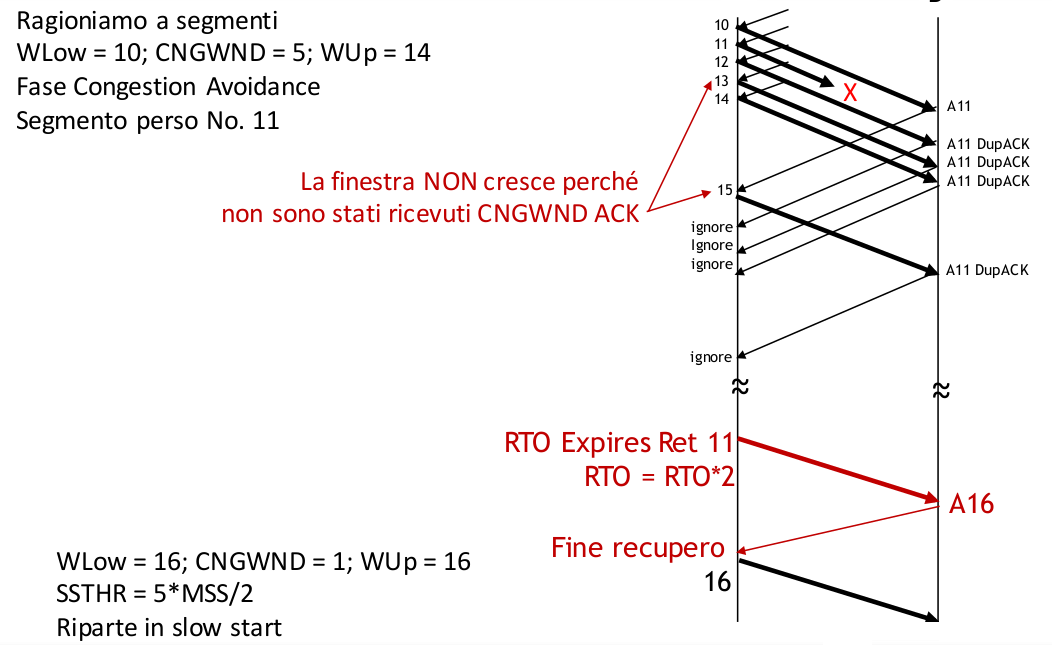
\includegraphics[scale=0.35]{livello_trasporto-img9.png}
\end{center}
Come si nota dall'esempio, alla perdita del segmento 11, il trasmettitore ricever\'a una serie di ACK duplicati con 
$SEQ=11$ che vengono ignorati; allo scadere del RTO ritrasmetter\'a il segmento 11 ricevendo come $ACK(SEQ)=16$, 
ovvero il prossimo numero di sequenza che il ricevitore si aspetta di ricevere.

Di seguito vengono riportati i grafici dell'invio effettivo dei segmenti ad ogni RTT. Il segmento in rosso \'e dove 
avviene la perdita. 

Si supponga che: $RTT=20ms, RTO=200ms, RCWND=40$ segmenti:
\begin{center}
	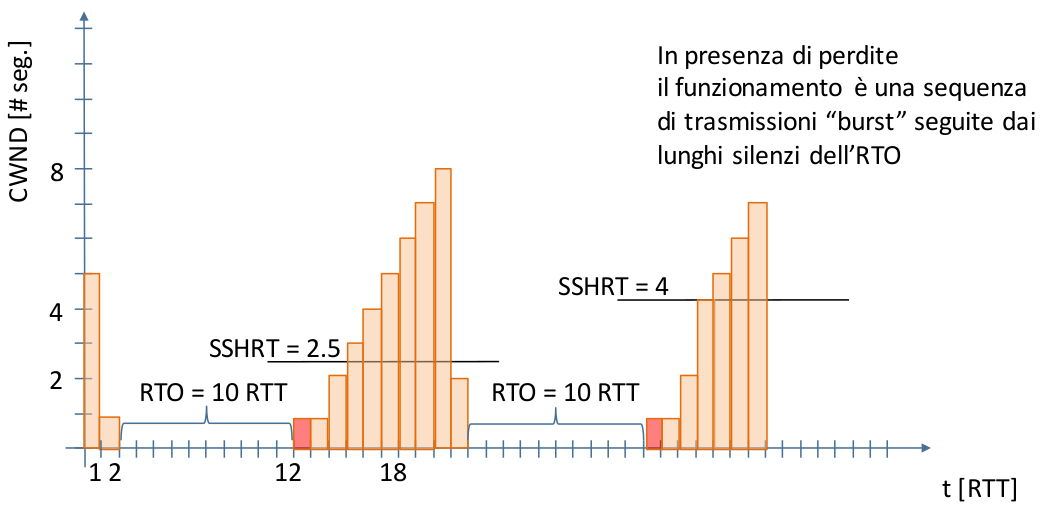
\includegraphics[scale=0.35]{livello_trasporto-img11.png}
\end{center}
Come si nota dal grafico, con il solo utilizzo del RTO, non \'e affatto efficiente, in quanto c'\'e bisogno di 18 RTT
prima che la CWND ritorni ad avere un numero di segmenti pari a prima della perdita e, nel caso di perdite multiple, 
si notano molti momenti di silenzio, dovuti al RTO, e a momenti di forte trasmissione a \textit{"burst"}.

Ovviamente questo andamento non \'e ottimale e non usa al meglio il mezzo trasmissivo.

\clearpage
\subsection{Recupero con Fast Retransmit}\label{recupero-delle-perdite-fast-retransmit}
Il secondo algoritmo usato da TCP \'e chiamato Fast Retransmit che, a differenza del precedente, utilizza
la seguente l'euristica: se si ricevono pi\'u di tre ACK duplicati, ovvero con numero di SEQ uguali, allora qualche 
segmento \'e andato perso e si pu\'o procedere alla ritrasmissione senza che scada nessuno timer. In effetti questa 
semplice idea migliora notevolmente l'utilizzo del mezzo trasmissivo e le prestazioni del trasferimento rispetto 
all'utilizzo puro del RTO.

La tecnica di recupero tramite RTO per\'o non \'e mai abbandonato del tutto, in quanto viene sempre inizializzato e, 
alla scadenza, si comporta esattamente come spiegato precedentemente.

L'algoritmo si comporta nel seguente modo quando riceve 3 ACK con lo stesso numero di sequenza:
\begin{enumerate}[noitemsep]
    \item $SSTRESH = CWND/2$: dimezza il valore della soglia di Slow Start
    \item $CWND = MSS$: viene impostata la finestra di congestione alla dimensione di un segmento
    \item Ritrasmette il primo segmento della finestra di congestione: per costruzione, il primo segmento \'e il 
          segmento non riscontrato
	\item Attende il riscontro: in questo caso pu\'o ricevere i seguenti tipi di ACK:
    \begin{itemize}[noitemsep]
    	\item se $ACK(SEQ) = W_{low}$ significa che \'e stato ricevuto ancora un ACK duplicato, quindi lo scarta
		\item se $W_{low} < ACK(SEQ) < W_{up}$ allora significa che ha riscontrato il segmento perso ed ha richiesto 
		      la ritrasmissione di un altro segmento della finestra, anch'esso perso; quindi viene spostato il bordo 
		      inferiore della finestra di trasmissione al numero di SEQ ricevuto: 
		      $W_{low} = ACK(SEQ)$ e $W_{up} = W_{low} + CWND$
	    \item se $ACK(SEQ) > W_{up}$ allora la ritrasmissione \'e andata a buon fine, tutti i segmenti
	          persi sono stati ricevuti e riscontrati quindi pu\'o riprendere la normale trasmissione
	\end{itemize}
	\item se scade il RTO si comporta come un recupero con puro RTO
\end{enumerate}
Nel momento in cui Fast Retransmit recupera l'informazione persa, la trasmissione riprende in Slow Start,
con i parametri impostati nel corso dell'algoritmo (SSTRESH al punto 1); limitando molto le
prestazioni dell'algoritmo. Questi semplici meccanismi si implementando di fatto la ritrasmissione selettiva 
dell'informazione persa.

\begin{center}
	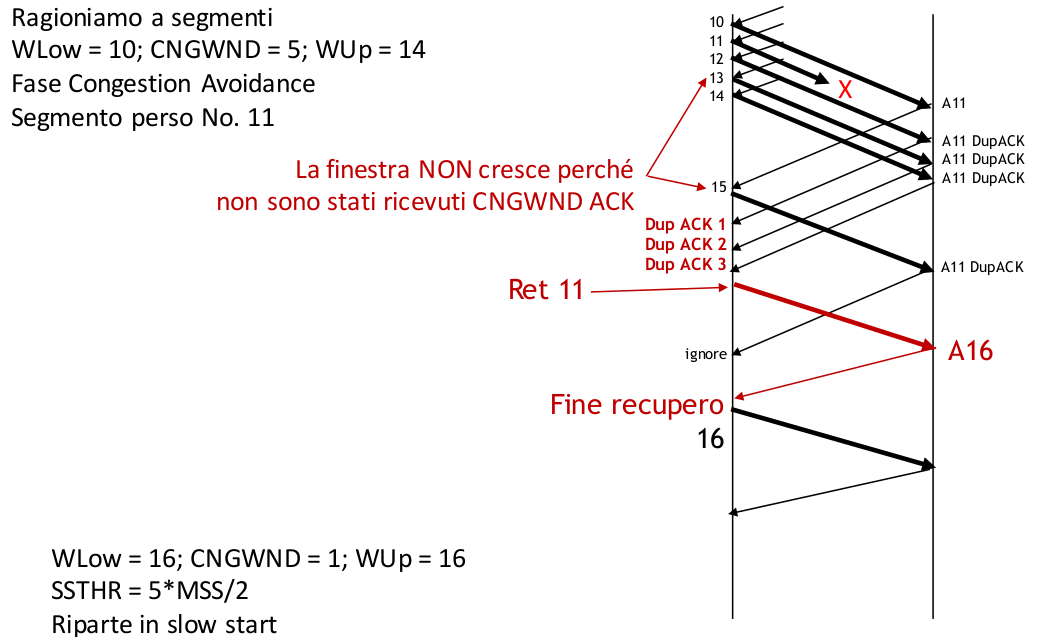
\includegraphics[scale=0.35]{livello_trasporto-img12.png}
\end{center}
Nell'esempio riportato si nota come il segmento con $SEQ=11$ venga perso, e alla ricezione dei 3 ACK
duplicati, si provveda alla sua riconsegna; ignorando l'ACK duplicato dopo la ritrasmissione, dovuto
al segmento con $SEQ=15$. 

Importante e sostanziale differenza rispetto ad RTO \'e che la ritrasmissione del segmento avviene dopo 
un solo RTT: si noti che, nel grafico sottostante, tra la perdita del segmento (barra rossa) e la ritrasmissione,
non \'e passato nessun RTT \textit{"vuoto"}, migliorando le prestazioni.

Si supponga che: $RTT=20ms, RTO=200ms, RCWND=40$ segmenti:

\begin{center}
	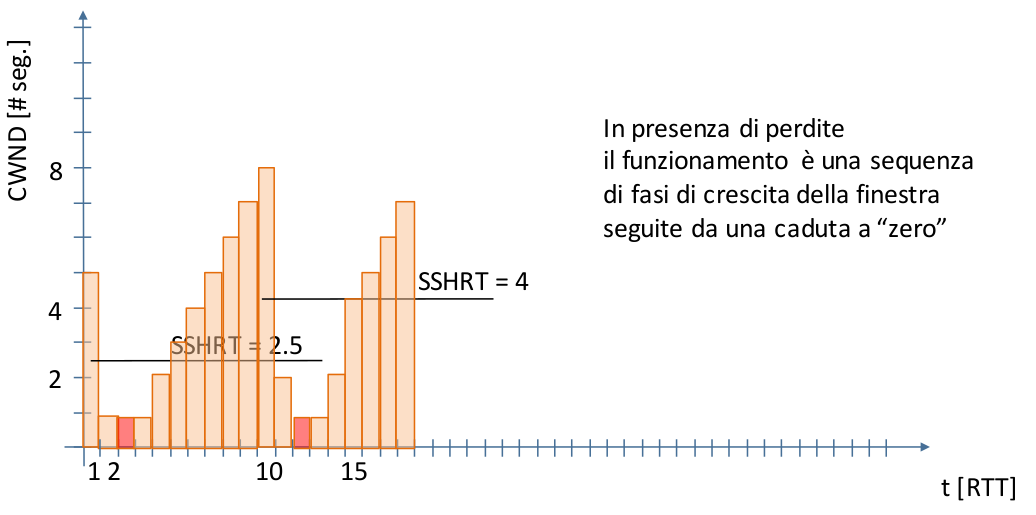
\includegraphics[scale=0.35]{livello_trasporto-img14.png}
\end{center}

Come si nota dal grafico, la finestra di congestione ritorna al suo valore precedente alla perdita solo
dopo 8 RTT, rispetto a 18 con RTO puro, con conseguente miglioramento del throughput.

\clearpage
\subsection{Recupero con Fast Recovery}\label{recupero-delle-perdite-fast-recovery}
L'idea di base per ottimizzare Fast Recovery \'e quella di non ricominciare da capo ogni volta, ma di impostare
la $CWND = SSTRESH$ e ricominciare in Congestion Avoidance; in questo modo si cerca di ottenere un oscillazione a 
\textit{"dente di sega"} dimezzandola in caso di perdite e incrementandola linearmente altrimenti.
\begin{center}
	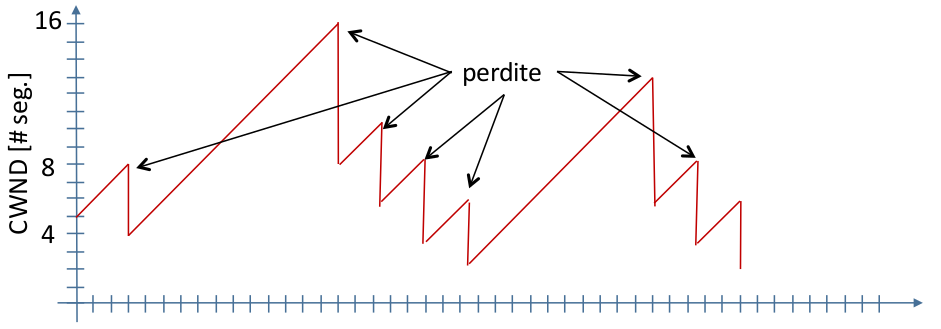
\includegraphics[scale=0.35]{livello_trasporto-img15.png}
\end{center}

L'algoritmo usato da Fast Recovery \'e uguale a Fast Retransmit per le modalit\'a in cui viene attivato (dopo 3 ACK 
duplicati) ma \'e pi\'u efficiente perch\'e consente di continuare l'invio di segmenti mentre st\'a ancora 
recuperando i segmenti persi:
\begin{enumerate}[noitemsep]
	\item $SSTRESH = CWND/2$: imposta la soglia di Slow Start a met\'a finestra di congestione
	\item Ritrasmette il primo segmento della finestra di congestione: per costruzione, il primo segmento \'e il 
	      segmento non riscontrato
	\item $CWND = SSTRESH + 3 \cdotp MSS$: imposta la finestra di congestione al valore della soglia di Slow Start
		  aggiungendo 3 segmenti, che sono i 3 ACK duplicati ricevuti all'inizio della perdita. Questo \'e dovuto 
		  dal fatto che il ricevitore ha ricevuto altri pacchetti (non quello che si aspettava) e gli ha 
		  riscontrati con ACK duplicati
	\item Attende il riscontro: in questo caso pu\'o ricevere i seguenti tipi di ACK:
	\begin{itemize}
		\item se $ACK(SEQ) = W_{low}$ significa che \'e stato ricevuto ancora un ACK duplicato, quindi 
		      $CWND = SSTRESH + MSS$, ovvero aumenta la finestra di congestione di un segmento, per i motivi del 
		      punto 3
		\item se $W_{low} < ACK(SEQ) < W_{up}$ allora significa che ha riscontrato il segmento perso ed ha richiesto 
		      la ritrasmissione di un altro segmento della finestra, anch'esso perso; quindi viene spostato il bordo 
	 	      inferiore della finestra di trasmissione al numero di SEQ ricevuto: 
	 	      $W_{low} = ACK(SEQ)$ e $W_{up} = W_{low} + CWND$     
		\item se $ACK(SEQ) > W_{up}$ allora la ritrasmissione \'e andata a buon fine, tutti i segmenti persi sono 
		      stati ricevuti e riscontrati quindi $CWND = SSTRESH$ e si pu\'o riprendere in Congestion Avoidance 
	\end{itemize}		
	\item se scade il RTO si comporta come un recupero con puro RTO
\end{enumerate}

\begin{center}
	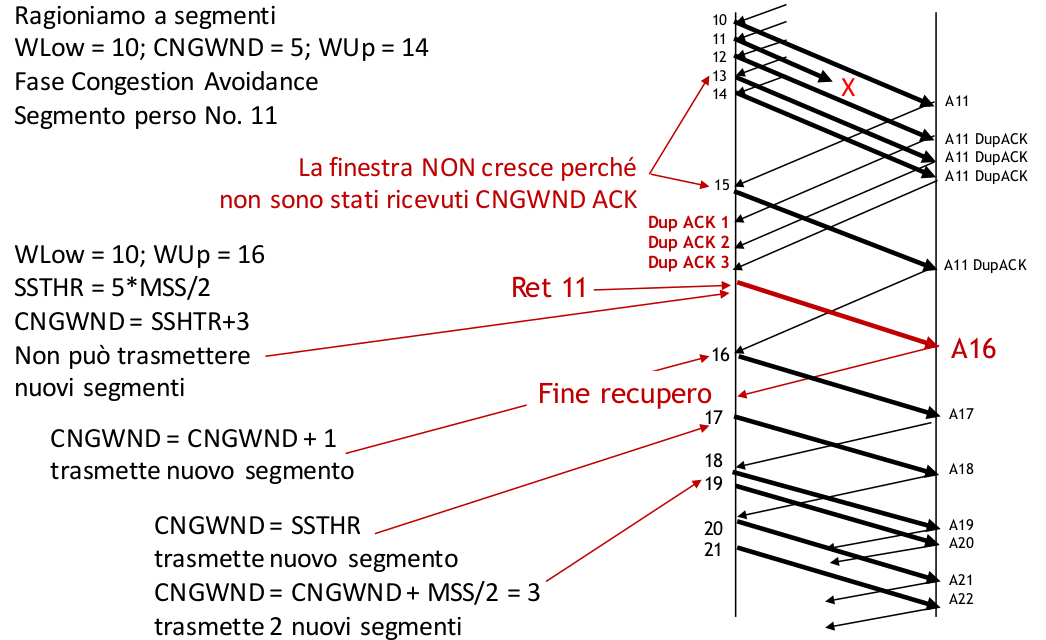
\includegraphics[scale=0.35]{livello_trasporto-img16.png}
\end{center}

Come si vede dall'esempio, dopo la ricezione di 3 ACK duplicati si procede alla ritrasmissione del segmento perso,
numero 11, ma quando ri riceve per la quarta volta ancora un riscontro duplicato, si fa crescere la finestra di 
congestione e si cerca di continuare a trasmettere segmenti (trasmissione del segmento numero 16).

Una volta ricevuto un ACK non duplicato che non \'e contenuto nell'attuale finestra di trasmissione, il che significa 
che ha riscontrato tutti i segmenti precedenti, si continua in Congestion Avoidance, incrementando linearmente la 
dimensione della finestra.

Di seguito vengono riportati i grafici dell'invio effettivo dei segmenti ad ogni RTT. Il segmento in rosso\'e dove 
avviene la perdita.

Si supponga che: $RTT=20ms, RTO=200ms, RCWND=40$ segmenti:

\begin{center}
	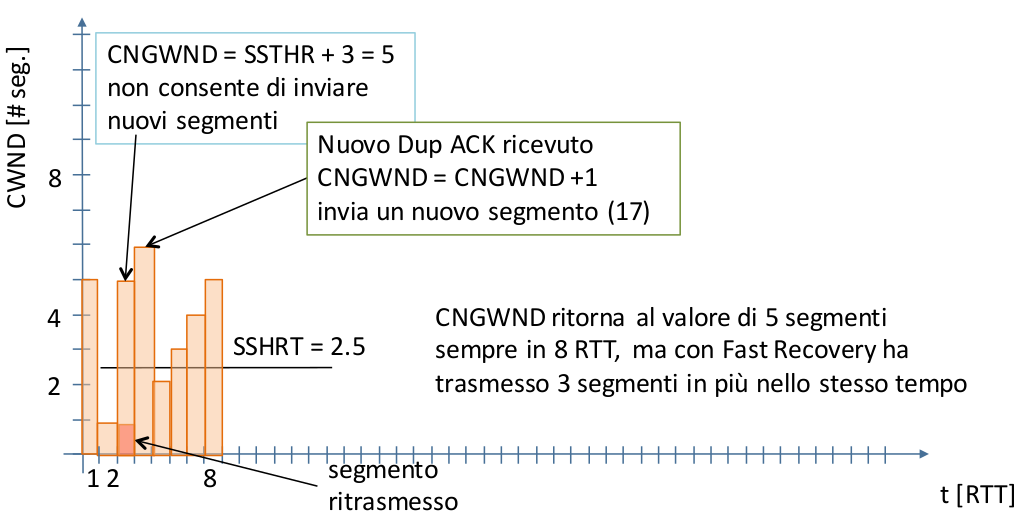
\includegraphics[scale=0.35]{livello_trasporto-img17.png}
\end{center}

Come si nota dal grafico soprastante, la situazione migliora molto rispetto a Fast Retransmit, in quanto in 8 RTT per 
recuperare la perdita si riesce ad inviare 3 nuovi segmenti. L'unico problema di Fast Recovery \'e quello della 
scadenza del RTO; infatti se la rete, o il ricevitore, sono particolarmente congestionate, il RTO continuer\'a a 
scadere, degradando le prestazioni.

\subsection{Riassumendo}\label{tcp-recupero-delle-perdite-riassumendo}
Riassumendo i meccanismi di recupero delle perdite:
\begin{itemize}[noitemsep]
    \item \textbf{RTO:} recupera un segmento alla volta. Funziona sempre ma spreca moltissime risorse
    \item \textbf{Fast Retransmit:} abbatte il tempo di recupero, consente di recuperare un segmento per RTT, 
          anzich\'e per RTO, ma \'e ancora inefficiente
    \item \textbf{Fast Recovery:} \'e il pi\'u efficiente ma, nel caso di perdite multiple, ricade nel caso di RTO
\end{itemize}

\subsection{Diagramma a Stati}\label{tcp-diagramma-a-stati}
Di seguito viene rappresentato il diagramma a stati di TCP in tutte le fasi della trasmissione dati:
\begin{center}
	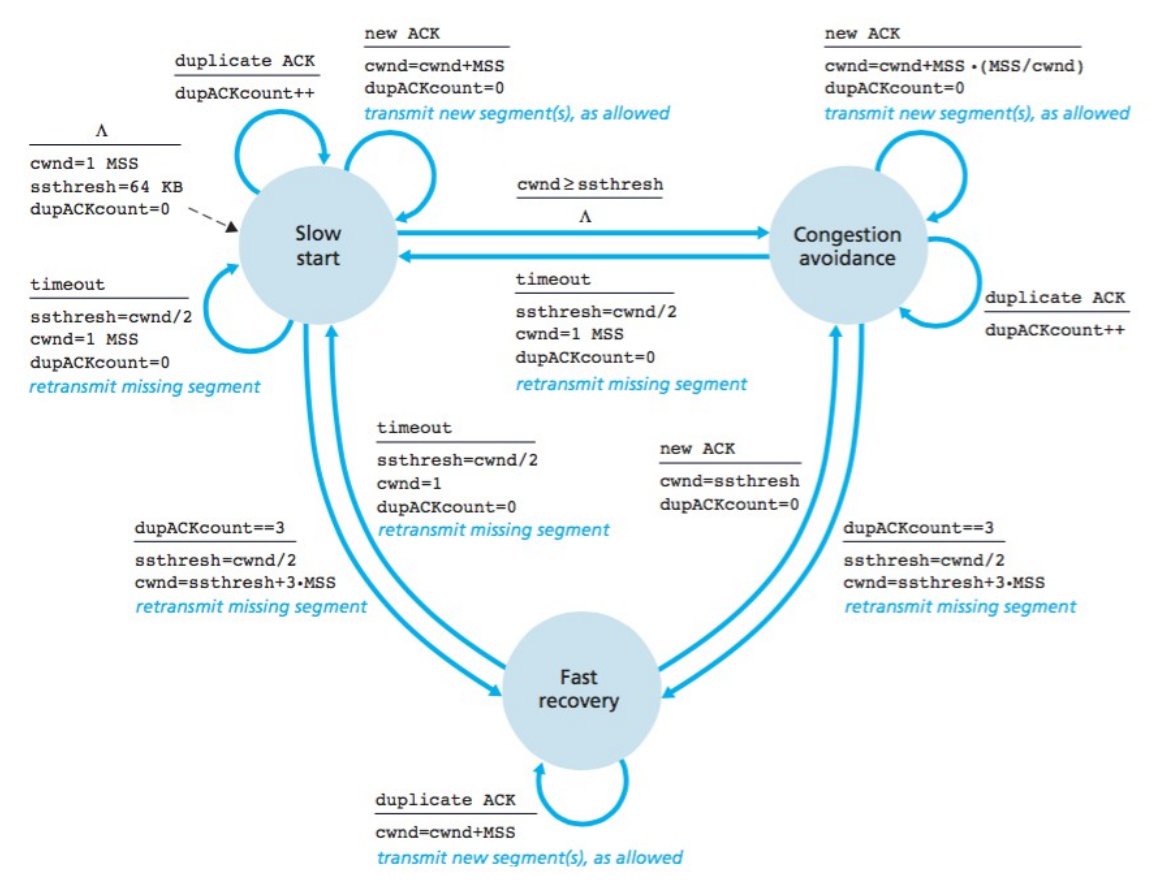
\includegraphics[scale=0.41]{livello_trasporto-img20.png}
\end{center}



\clearpage
\section{UPD}\label{udp}
UDP \textit{(User Datagram Protocol)} \'e un protocollo leggero e veloce, in quanto fornisce un servizio di solo 
invio di segmenti senza conferma di ricezione e senza bisogno di instaurare una connessione tra le entit\'a 
coinvolte; per questo viene definito \textit{non connesso-non confermato}.

Questo porta alcuni svantaggi, ad esempio non gestisce il controllo di flusso o la ritrasmissione dei segmenti 
corrotti o mai arrivati, ma demanda alle applicazioni che lo utilizzano l'implementazione di tali meccanismi.

D'altro canto per\'o \'e l'unico protocollo che permette a tutte le applicazioni in real-time di funzionare: basti 
pensare alla comunicazione audio/video, in questo caso non e' importante la consegna in sequenza e completa dei 
segmenti, in quanto si tende ad accettare una certa tolleranza di perdita a fronte di una comunicazione il pi\'u 
possibile fluida e in tempo reale.

Il segmento UDP \'e composto:
\begin{center}
\begin{bytefield}[boxformatting={\centering},bitwidth=1.0em, bitheight=2em]{32}
	\bitheader{0,15,16,31} \\
	\begin{rightwordgroup}{header\\8 byte}
		\bitbox{16}{Porta Sorgente} & \bitbox{16}{Porta Destinazione}\\
		\bitbox{16}{Lunghezza}      & \bitbox{16}{Checksum}
	\end{rightwordgroup}\\
	\begin{rightwordgroup}{payload\\0-65527\\byte}
		\wordbox{4}{Dati}
	\end{rightwordgroup}
\end{bytefield}
\end{center}

\begin{itemize}[noitemsep]
    \item \textbf{Porta Sorgente e Destinazione}: numero di porta sorgente e destinazione
    \item \textbf{Lunghezza}: valore in byte che identifica la lunghezza dell'intero segmento
    \item \textbf{Checksum}: campo per il controllo degli errori per l'intestazione e i dati
    \item \textbf{Dati}: i dati che trasporta il segmento
\end{itemize}

\paragraph{Perch\'e non usare direttamente il livello di Rete sottostante ?} Non \'e possibile in quanto non gestisce 
la comunicazione end-to-end, infatti nell'intestazione del pacchetto IP non \'e presente la porta sorgente e 
destinazione. 

\end{document}